% Source for the figure of StealablePriorityQueue (sec. 24.11): the two
% heaps of an owner that pushed the keys 1 to 8, in the order of a 4-ary
% heap; serve() moves into the offer the heap whose least key is not the
% least, and a thief claims it by an exchange and deals its pairs to two
% heaps of its own. Build: make figures (in ../build).
\documentclass[border=4pt]{standalone}
\usepackage[T1]{fontenc}
\usepackage{lmodern}
\usepackage{amsmath,amssymb}
\usepackage{tikz}
\usepackage{lamalunga}
% tikz-ads.tex: the TikZ styles shared by the figures of the memory of the
% manual, \input by each standalone figure: a cell of a vector (cell), the
% cell that an operation touches (touched), a free cell (free), a node of a
% linked structure (node), the labels of indices (index) and of variables
% (var), a pointer (ptr), and \cells and \indices to draw a row of cells.
\usetikzlibrary{arrows.meta,positioning,calc,fit,shapes.multipart}
\definecolor{adsTouched}{RGB}{214,196,236}
\definecolor{adsFree}{RGB}{236,236,236}
\tikzset{
  ads/.style={>={Stealth[length=2mm]},font=\small,
              every node/.append style={inner sep=0pt}},
  cell/.style={draw,minimum width=7mm,minimum height=7mm,
               font=\small\ttfamily,outer sep=0pt},
  touched/.style={cell,fill=adsTouched},
  free/.style={cell,fill=adsFree,text=black!45},
  node/.style={draw,rounded corners=1pt,minimum width=8mm,
               minimum height=6mm,font=\small\ttfamily},
  index/.style={font=\scriptsize\ttfamily,text=black!60},
  var/.style={font=\small\itshape},
  ptr/.style={->,thick}
}
% \cells{name}{x,y}{list}: a row of cells, the first at (x,y), named
% name-0, name-1, ...; each item is text/style, the style one of cell,
% touched and free (e.g., {a/cell,e/touched,/free})
\newcommand{\cells}[3]{%
  \foreach \v/\s [count=\i from 0] in {#3}
    \node[\s] (#1-\i) at ($(#2)+(\i*7mm,0)$) {\v};}
% \indices{name}{n}: the indices 0 .. n-1 under the cells of name
\newcommand{\indices}[2]{%
  \foreach \i in {0,...,\numexpr#2-1\relax}
    \node[index,below=1.2mm of #1-\i] {\i};}

\begin{document}
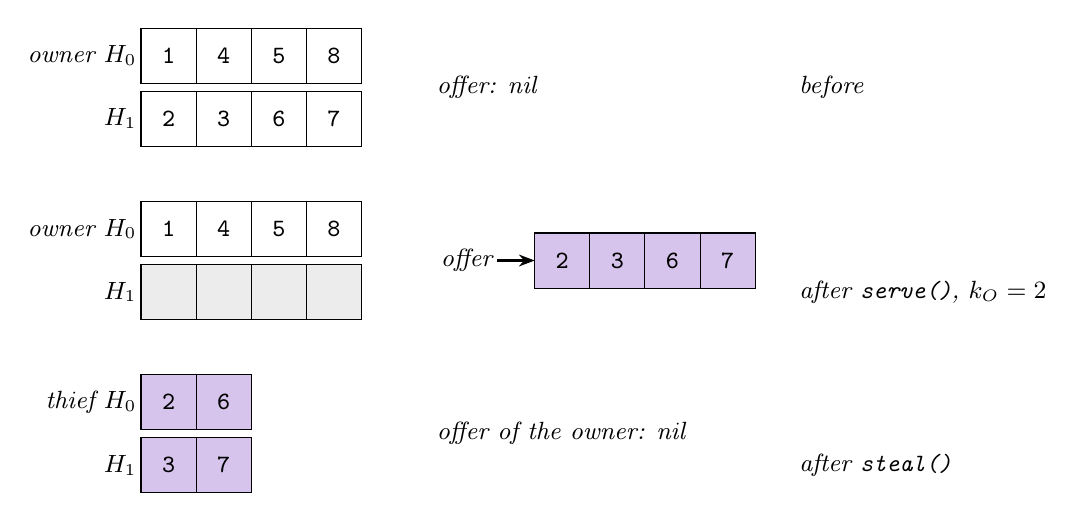
\begin{tikzpicture}[ads]
  \node[var,anchor=east] at (-4mm,0) {owner $H_0$};
  \cells{a}{0,0}{1/cell,4/cell,5/cell,8/cell}
  \node[var,anchor=east] at (-4mm,-8mm) {$H_1$};
  \cells{b}{0,-8mm}{2/cell,3/cell,6/cell,7/cell}
  \node[var,anchor=west] at (34mm,-4mm) {offer: nil};
  \node[var,anchor=west] at (80mm,-4mm) {before};
  \node[var,anchor=east] at (-4mm,-22mm) {owner $H_0$};
  \cells{c}{0,-22mm}{1/cell,4/cell,5/cell,8/cell}
  \node[var,anchor=east] at (-4mm,-30mm) {$H_1$};
  \cells{d}{0,-30mm}{/free,/free,/free,/free}
  \node[var,anchor=west,inner sep=1.5pt] (of) at (34mm,-26mm) {offer};
  \cells{e}{50mm,-26mm}{2/touched,3/touched,6/touched,7/touched}
  \draw[ptr] (of) -- (e-0.west);
  \node[var,anchor=west] at (80mm,-30mm) {after \texttt{serve()}, $k_O = 2$};
  \node[var,anchor=east] at (-4mm,-44mm) {thief $H_0$};
  \cells{f}{0,-44mm}{2/touched,6/touched}
  \node[var,anchor=east] at (-4mm,-52mm) {$H_1$};
  \cells{g}{0,-52mm}{3/touched,7/touched}
  \node[var,anchor=west] at (34mm,-48mm) {offer of the owner: nil};
  \node[var,anchor=west] at (80mm,-52mm) {after \texttt{steal()}};
\end{tikzpicture}
\end{document}
